\section{The Large Hadron Collider and the CMS Detector}

\emph{%
This section covers the Large Hadron Collider and the CMS detector.
% 
}


\subsection{The Large Hadron Collider}

The Large Hadron Collider at CERN is the largest particle accelerator with the highest center-of-mass energy to date.
% 
It is the final stage in a series of accelerators which are part of the CERN accelerator complex, which is illustrated in Fig.~\ref{fig:cernacceleratorcomplex}.
% 
The LHC is built partially in Switzerland and in France, and it is located about 100\unit{m} underground.
% 
Its design corresponds to a \textit{storage ring}, in which particles are kept in a circular trajectory for an extended period of time using powerful superconducting magnets.
% 
The achievable center-of-mass energy for proton-proton collisions, the primary research mode for the LHC, depends on the magnetic field strength of these 1232 bending magnets (about 8.3\unit{T}~\cite{lhc}) and the radius of the ring (about 27\unit{km}).
% 
The latest data from the LHC, including the data used in this thesis, was collected at $\sqrt{s}=13\TeV$.
% 
The LHC employs 16 radiofrequency (RF) cavities in order to create tight particle bunches and to accelerate particles from the insertion energy of about 450\GeV to 6.5\TeV.


\begin{figure}[hbtp]
  \begin{center}
    \includegraphics[width=\linewidth]{img/detector/cernacceleratorcomplex_small.png}
    \caption{
        The CERN accelerator complex. Taken from Ref.~\cite{cernacceleratorcomplex}.
        }
    \label{fig:cernacceleratorcomplex}
  \end{center}
\end{figure}


Of the many detectors associated with the CERN accelerator complex, the four most prominent ones are the CMS detector, the ATLAS detector, the LHCb detector, and the ALICE detector.
% 
The CMS and ATLAS detectors are both general-purpose detectors, with a similar physics program meant to yield comparable measurements.
% 
This thesis concerns data from the CMS experiment, and the structure of its detector is treated in more detail in Section~\ref{sec:cmsdetector}.


For any particle physics process, the rate of events $\mathrm{d}R/\mathrm{d}t$ is given by
% 
\begin{linenomath*}
\begin{equation}
\frac{\mathrm{d}R}{\mathrm{d}t} = \sigma \, L_\text{inst}
\,,
\end{equation}
\end{linenomath*}
% 
where $\sigma$ is the cross section of the process and $L_\text{inst}$ is the instantaneous luminosity.
% 
For a given center-of-mass energy, $\sigma$ is a constant; the instantaneous luminosity, however, is a machine quantity that is to be optimized in the design of an accelerator.
% 
For two colliding beams containing an equal number of particles $N$ that are Gaussian-distributed in the plane perpendicular to the direction of motion with a beam width $\sigma_\text{beam}$, the instantaneous luminosity is given by~\cite{griffiths}
% 
\begin{linenomath*}
\begin{equation}
L_\text{inst} =
\frac{
    N^2 f N_b 
    }{
    4 \pi \sigma_\text{beam}^2
    }
\,,
\end{equation}
\end{linenomath*}
% 
where $f$ is the revolution frequency and $N_b$ is the number of bunches.
% 
The \textit{integrated luminosity} $L$ is given by the integral of the instantaneous luminosity over time and is typically expressed in units of \fbinv.
% 
It is the typical quantity employed for indicating the size of a collection of data.


At the time of writing, the LHC has just finished its second data-taking run, colloquially referred to as `Run 2'.
% 
Combined with the first data-taking run, the LHC has delivered almost 200\fbinv, and is expected to deliver around 300\fbinv by the end of the third data-taking run.
% 
The evolution of the delivered luminosity and the collected luminosity by the CMS detector is shown in Fig.~\ref{fig:cmslumi}.

\begin{figure}[hbtp]
  \begin{center}
    \includegraphics[width=0.7\linewidth]{img/detector/cmslumi.pdf}
    \caption{
        Cumulative delivered and recorded luminosity at the CMS detector versus time for 2010-2012 and 2015-2018.
        % 
        Only proton-proton collision data is taken into account.
        % 
        Taken from Ref.~\cite{cmslumi}.
        }
    \label{fig:cmslumi}
  \end{center}
\end{figure}


\subsection{The CMS detector}
\label{sec:cmsdetector}

As a general-purpose detector, the CMS detector was designed to be able to detect most SM particles over a large range of energy scales.
% 
The cylindrical shape, with the beam axis at its center, provides a nearly complete solid angle coverage, up to a pseudo-rapidity of $\eta \leq 3.0$.
% 
The components of the detector are illustrated in Fig.~\ref{fig:cmsgeometry}; starting from the beam axis, the first detector is the silicon tracker, followed by the electromagnetic calorimeter (ECAL), and the hadron calorimeter (HCAL).
% 
These detectors are enclosed in the superconducting solenoid magnet, which delivers a magnetic field strength of 3.8\unit{T}, is cooled with liquid helium, and is the largest superconducting solenoid to date.
% 
With its 14000 tonnes and its length of 28.7\unit{m}, `Compact Muon Solenoid' seems to be a misnomer at first glance, but for the range of detector applications it provides, the CMS detector can in fact be considered relatively compact.
% 
Of the stable SM particles listed in Section~\ref{sec:sm}, the CMS detector detects electrons, photons, stable hadrons, and muons; the typical trajectories of these particles are illustrated in Fig.~\ref{fig:cmsslice}.
% 
A full description of the CMS detector can be found in Ref.~\cite{Chatrchyan:2008zzk}.


\begin{figure}[hbtp]
  \begin{center}
    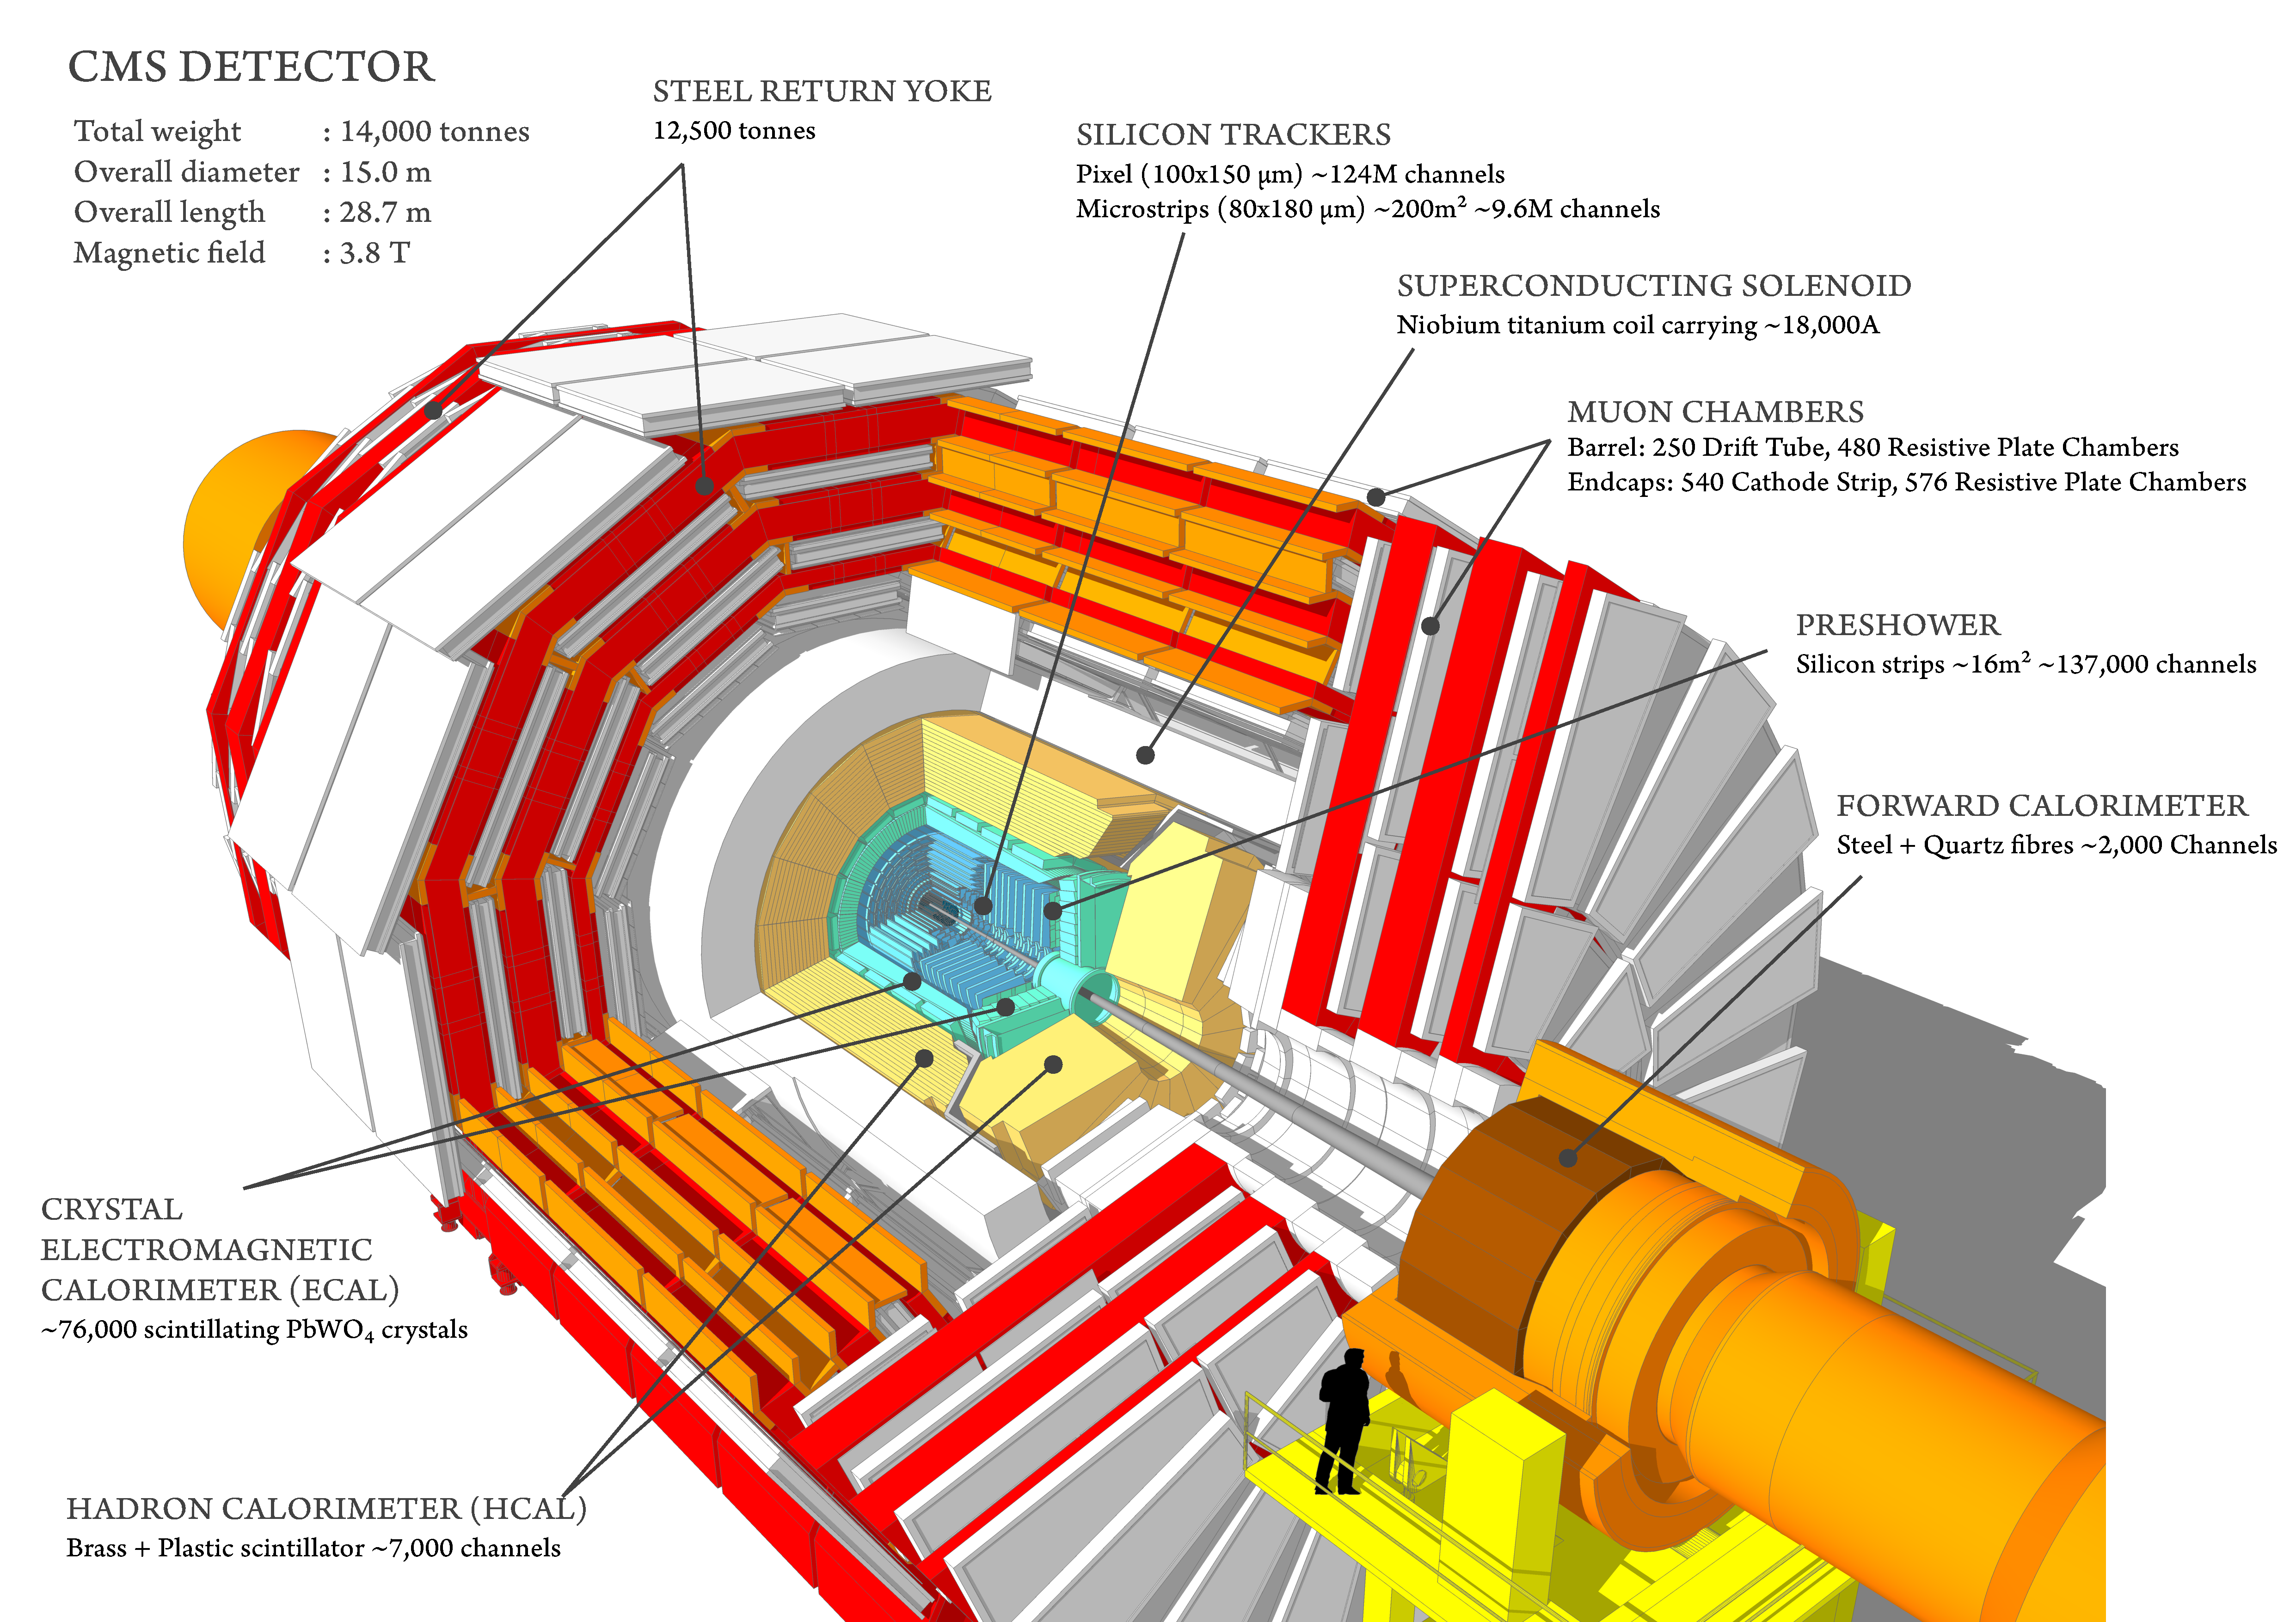
\includegraphics[width=\linewidth]{img/detector/cmsgeometry.pdf}
    \caption{
        A 3-dimensional view of the CMS detector with a cut-out section.
        % 
        Taken from Ref.~\cite{Sakuma:2013jqa}.
        }
    \label{fig:cmsgeometry}
  \end{center}
\end{figure}


\begin{figure}[hbtp]
  \begin{center}
    \includegraphics[width=\linewidth]{img/detector/cmsslice.png}
    \caption{
        A transverse slice of the CMS detector.
        % 
        Taken from Ref.~\cite{cmsslice}.
        }
    \label{fig:cmsslice}
  \end{center}
\end{figure}


\subsubsection{The inner tracking system}

The inner tracking system, consisting of a pixel detector surrounded by a silicon strips detector, measures the trajectories of charged particles and reconstructs secondary vertices.
% 
It is designed once again designed cylindrically, with a length of 5.8\unit{m} and a diameter of 2.5\unit{m}, and is able to perform measurements up to $\abs{\eta} \leq 2.5$.
% 
As high radiation levels are part of the operating environment, the tracker is designed to be radiation hard.
%
An important design parameter of the inner tracker is the material budget, which directly affects the achievable resolution of the other subdetector systems; the complete inner tracker corresponds to 0.4 radiation lengths in the central region, and increases up to almost 2 radiation lengths in the forward regions~\cite{Chatrchyan:2008zzk}.
% 
The trajectory is precisely measured with 11 to 17 trajectory points, which requires 66 million pixels and 91 million strips in the pixel and strips detectors, respectively.
% 
The inner tracker is the most important subsystem for low-energy particles; for single muons up to 100\GeV and $\abs{\eta} \leq 1.6$, the \pt resolution is around 1-2\%.


\subsubsection{The electromagnetic calorimeter}

The electromagnetic calorimeter, starting at an inner radius of 1.3\unit{m}, is responsible for the energy measurement of charged particles, and is in particular important for the high-precision measurement of the energy of photons and electrons.
% 
It consists of 61200 lead-tungstate crystals in the barrel region, which have a length of 230\unit{mm} and correspond to 25.8 radiation lengths.
% 
Lead-tungstate crystals have a short scintillation time, are optically clear, and relatively radiation hard.
% 
The barrel region is organized into 36 \textit{supermodules}, each of which consists of 4 \textit{modules}.
% 
The modules further removed from the interaction point have their crystals tilted, so that the front face of the crystal is aimed towards the interaction point.
% 
The barrel covers the measurements up to $\abs{\eta} \leq 1.479$.
% 
The forward regions are covered by two endcaps approximately 3\unit{m} from the interaction point in the longitudinal direction, which extend up to $\abs{\eta} \leq 3.0$ and consist of 7324 identical crystals each.
% 
Also these crystals are slanted so that the small front face of the crystal points to the interaction point.
% 
The endcaps are prefaced by the 20\unit{cm} thick \textit{preshower}, whose primary purpose is the enhanced identification of neutral pions in the forward region.
% 
The preshower is a sampling calorimeter that consists of two layers, each containing a lead plate (which initiates electromagnetic showers) and a silicon strip sensor (which measures the deposited energy and the transverse shower profile).


The energy resolution



\subsubsection{The hadron calorimeter}

\tk{TODO}


\subsubsection{The muon system}

\tk{TODO}


\subsubsection{The trigger and data acquisition systems}

\tk{TODO}
